\label{1.2.10}

\textit{The Cone Over a Projective Variety} (\ref{fig1.2.3}). Let $Y \subseteq \P^n$ be a nonempty algebraic set, and let $\theta :\A^{n + 1} -
\{(0, \dots ,0)\} \longrightarrow \P^n$ be the map which sends the point with affine coordinates $(a_0, \dots, a_n)$ to the point with homogeneous coordinates $(a_0 , \dots ,a_n)$· We define the \textit{affine cone} over $Y$ to be

\[
    C(Y) = \theta^{- 1}[Y] \cup \{(0, \dots ,0)\}.
\]

\begin{enumerate}[label = (\alph*)]
    \item Show that $C(Y)$ is an algebraic set in $\A^{n + 1}$, whose ideal is equal to $I(Y)$, considered as an ordinary ideal in $k[x_0 , \dots x_n]$.
    
    \item $C(Y)$ is irreducible if and only if $Y$ is.
    
    \item $\dim C(Y) = \dim Y + 1$.
\end{enumerate}

Sometimes we consider the projective closure $\overline{C(Y)}$ of $C(Y)$ in $\P^{n + 1}$ . This is called the \textit{projective cone} over $Y$.


\begin{figure}
    \centering
    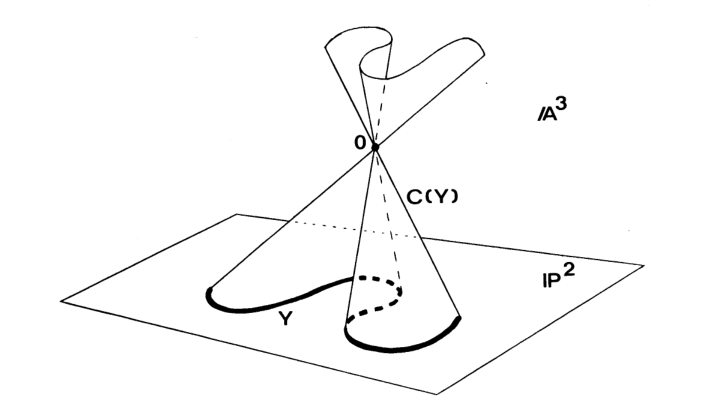
\includegraphics{Fig 01}
    \caption{The cone over a curve in $\P^2$.}
    \label{fig1.2.3}
\end{figure}

\begin{proof}
    \begin{enumerate}[label= (\alph*)]
        \item Let $I = I(Y)$, so that $Y = Z(I)$. We seek to compute $\theta^{-1}[Z(I)]$. Indeed, we claim that this is precisely $V(I) - 0$. If $(a_0, \dots, a_n) \in V(I) - 0$ then $\theta(a_0, \dots, a_n) = [a_0 : \dots : a_n] \in \P^n$. Let $f \in I^h$. Then $f(a_0, \dots, a_n) = 0$ so indeed, $f([a_0 : \dots : a_n]) = 0$ and $\theta(a_0, \dots, a_n) \in Z(I)$. Hence, $V(I) - 0 \subseteq \theta^{-1}[Z(I)]$. Conversely, let $\theta(a_0, \dots, a_n) \in Z(I)$. Then of course $(a_0), \dots, a_n) \neq 0$. Let $f \in I$ and write $f = \sum f_e$ the homogeneous decomposition. As $I = I(Y)$ is homogeneous, each $f_e \in I^h$. Then as $[a_0 : \dots : a_n] \in Z(I)$, we have that $f_e(a_0, \dots, a_n) = 0$ for all $e$. Hence, $f(a_0, \dots, a_n) = 0$ and we have computed $\theta^{-1}[Z(I)] = V(I) - 0$.

        Additionally, every $f \in I^h$ vanishes on $0$. Furthermore, $Y \neq \emptyset$ so $1 \notin I$. Hence, every nonzero element of $I$ is the sum of homogeneous elements of $I$, all of which vanish on $0$, so every element of $I$ vanishes on $0$. Thus, we conclude that $V(I) = \theta^{-1}[Z(I)] \cup 0$. Then $J(C(Y)) = I$ by the Nullstellensatz.

        \item $C(Y)$ is irreducible iff $I(C(Y)) = I(Y)$ irreducible iff $Y$ is irreducible.

        \item $\dim C(Y) = \dim k[x_0, \dots, x_n] / I(C(Y)) = \dim k[x_0, \dots, x_n] / I(Y) = \dim Y + 1$.
    \end{enumerate}
\end{proof}
